\begin{table}[tb]
    \caption{
      Performance comparison in linear evaluation protocol
      on NTU 60, NTU 120, and PKU MMD datasets.
      \textit{Single-stream} refers to Joint,
      while \textit{Three-stream} denotes Joint+Motion+Bone.
    }
    \centering
    \setlength{\tabcolsep}{4pt} % 增大列与列之间的水平间距
    \begin{tabular}{l c c c c c c}
      \toprule
      \multirow{2}{*}{Method} &
      \multirow{2}{*}{Input} &
      \multicolumn{2}{c}{NTU 60} &
      \multicolumn{2}{c}{NTU 120} &
      PKU II\\
      % & & XSub(\%) & XView(\%) & XSub(\%) & XSet(\%) & XSub(\%) \\
      & & XSub & XView & XSub & XSet & XSub \\
      \midrule
      \rowcolor{Gray!20} \multicolumn{7}{l}{\textit{Other pretext tasks:}} \\
      LongTGAN \cite{zheng2018unsupervised} & Single-stream & 39.1 & 48.1 & - & - & 26.0 \\
      P\&C \cite{su2020predict} & Single-stream & 50.7 & 75.3 & 42.7 & 41.7 & 25.5 \\
      \midrule
      \rowcolor{Gray!20} \multicolumn{7}{l}{\textit{Contrastive Learning:}} \\
      CrosSCLR \cite{li20213d} & Three-stream & 77.8 & 83.4 & 67.9 & 66.7 & 21.2 \\
      AimCLR \cite{guo2022contrastive} & Three-stream & 78.9 & 83.8 & 68.2  & 68.8 & 39.5 \\
      CPM \cite{zhang2022contrastive} & Single-stream & 78.7 & 84.9 & 68.7 & 69.6 & - \\
      PSTL \cite{Zhou2023SelfsupervisedAR} & Three-stream & 79.1 & 83.8 & 69.2 & 70.3 & 52.3 \\
      CMD \cite{mao2022cmd} & Single-stream & 79.4 & 86.9 & 70.3 & 71.5 & - \\
      HaLP \cite{shah2023halp} & Single-stream & 79.7 & 86.8 & 71.1 & 72.2 & 43.5 \\
      HiCo-Transformer \cite{hico2023} & Single-stream & 81.1 & 88.6 & 72.8 & 74.1 & 49.4 \\
      SkeAttnCLR \cite{Hua2023SkeAttnCLR} & Three-stream & 82.0 & 86.5 & 77.1 & 80.0 & 55.5 \\
      ActCLR \cite{lin2023actionlet} & Three-stream & 84.3 & 88.8 & 74.3 & 75.7 & - \\
      \midrule
      \rowcolor{Gray!20} \multicolumn{7}{l}{\textit{Masked Prediction:}} \\
      SkeletonMAE \cite{yan2023skeletonmae} & Single-stream & 74.8 & 77.7 & 72.5 & 73.5 & 36.1 \\
      MAMP \cite{mao2023masked} & Single-stream & 84.9 & 89.1 & 78.6 & 79.1 & 53.8 \\
      \textbf{Skeleton2vec(Ours)} & Single-stream & \textbf{85.7} & \textbf{90.3} & \textbf{79.7} & \textbf{81.3} & \textbf{55.6} \\
      \bottomrule
    \end{tabular}
    \label{tab:linear}
\end{table}

\section{Experiments}
\subsection{Datasets}
We evaluate our method on three large-scale 3D skeleton-based action recognition
datasets: NTU RGB+D 60, NTU RGB+D 120, and PKU Multi-Modality Dataset (PKUMMD).

NTU RGB+D 60 \cite{shahroudy2016ntu} contains 56,880 skeleton sequences across 60
action categories performed by 40 subjects. We follow the recommended cross-subject
and cross-view evaluation protocols. For cross-subject, sequences from 20 subjects
are used for training and the rest are used for testing. For cross-view, training
samples are from cameras 2 and 3, while testing samples are from camera 1. 

NTU RGB+D 120 \cite{liu2019ntu} is an extension of NTU RGB+D 60 with 114,480
skeleton sequences across 120 action categories performed by 106 subjects.
The authors also propose a more challenging cross-setup evaluation protocol, where
sequences are divided into 32 setups based on camera distance and background. Samples
from 16 setups are used for training and the rest are used for testing.

PKUMMD \cite{liu2017pku} contains nearly 20,000 skeleton sequences across 52 action
categories. We adopt the cross-subject protocol, where training and testing sets are
split based on subject ID. PKUMMD consists of two parts: PKU-I and PKU-II. PKU-II is
more challenging due to larger view variations that introduce more skeleton noise.
For PKU-II, there are 5,332 sequences for training and 1,613 for testing.

\subsection{Settings}
\noindent \textbf{Data Processing:}
We employed the data preprocessing method from DG-STGCN \cite{duan2022dg} to apply
uniform sampling to a given skeleton sequence, generating subsequences as training
samples. The number of frames $T_{s}$ for sampling is set to 90.
During the training, we applied random rotation as data augmentation on the
sampled subsequences to enhance robustness against view variation. During the testing,
we averaged the scores of 10 subsequences to predict the class.

\noindent \textbf{Network Architecture:}
We adopted the same network architecture setting as MAMP \cite{mao2023masked}, with the
encoder layers $L_{e}$ set to 8, decoder layers $L_{d}$ set to 3, embedding dimension
set to 256, the number of heads in the multi-head self-attention module set to 8, and
the hidden dimension of the feed-forward network set to 1024. For Joint Embedding,
the length $l$ of each segment is set to 3.

\noindent \textbf{Pre-training:}
In the pre-training, the initial value of the EMA parameter $\tau$ is set to 0.9999.
The masking ratio $m$ of the input sequence is set to 90\%.
The tube length $\alpha$ for motion-aware multi-tube masking is set to 5,
and the sampling parameter $\beta$ is set to 0.1. We utilized the AdamW optimizer
with weight decay of 0.05 and betas (0.9, 0.95). The model was trained for a total of
600 epochs, with the learning rate linearly increasing to 1e-3 during the first 20
warmup epochs, and then decaying to 1e-5 according to a cosine decay schedule.
Our model was trained on 2 RTX 4090 GPUs, with a total batch size of 128.

\subsection{Evaluation and Comparison}
\noindent \textbf{Linear Evaluation:}
In the linear evaluation protocol, the parameters of the pre-trained encoder are
fixed to extract features. A trainable linear classifier is then applied for
classification. We train for 100 epochs in total using SGD optimizer with momentum of
0.9 and batch size of 256.
The initial learning rate is set to 0.1 and is decreased to 0 following a
cosine decay schedule.
Our results are evaluated on three datasets: NTU-60, NTU-120, and PKU-MMD.
Comparison with the latest methods reveals the superiority of our proposed Skeleton2vec,
as illustrated in \cref{tab:linear}. Notably, in contrast to contrastive learning
methods, Skeleton2vec, employing the masked prediction approach, demonstrates significant advantages.
Furthermore, Skeleton2vec outperforms other masked prediction methods across all datasets.
Particularly, on the NTU-60 XView and NTU-120 XSet datasets, Skeleton2vec exhibits
superior performance over the previously state-of-the-art method MAMP by 1.2\% and 2.2\%,
respectively, highlighting the strength of our contextualized prediction targets.

\begin{table}[tb]
    \caption{
      Performance comparison in the semi-supervised protocol on NTU 60 datasets.
      We averaged the results of five runs as the final performance.
    }
    \centering
    \setlength{\tabcolsep}{4pt} % 增大列与列之间的水平间距
    \begin{tabular}{l c c c c c}
      \toprule
      \multirow{3}{*}{Method} &
      \multirow{2}{*}{Input} &
      \multicolumn{4}{c}{NTU 60} \\
      & & \multicolumn{2}{c}{XSub} & \multicolumn{2}{c}{XView} \\
      & & (1\%) & (10\%) & (1\%) & (10\%) \\
      \midrule
      \rowcolor{Gray!20} \multicolumn{6}{l}{\textit{Other pretext tasks:}} \\
      LongTGAN \cite{zheng2018unsupervised} & Single-stream & 35.2 & 62.0 & - & - \\
      MS2L \cite{lin2020ms2l} & Single-stream & 33.1 & 65.1 & - & - \\
      \rowcolor{Gray!20} \multicolumn{6}{l}{\textit{Contrastive Learning:}} \\
      ISC \cite{thoker2021skeleton} & Single-stream & 35.7 & 65.9 & 38.1 & 72.5 \\
      3s-CrosSCLR \cite{li20213d} & Three-stream & 51.1 & 74.4 & 50.0 & 77.8 \\
      3s-Colorization \cite{yang2021skeleton} & Three-stream & 48.3 & 71.7 & 52.5 & 78.9 \\
      3s-Hi-TRS \cite{chen2022hierarchically} & Three-stream & 49.3 & 77.7 & 51.5 & 81.1 \\
      3s-AimCLR \cite{guo2022contrastive} & Three-stream & 54.8 & 78.2 & 54.3 & 81.6 \\
      3s-CMD \cite{mao2022cmd} & Three-stream & 55.6 & 79.0 & 55.5 & 82.4 \\
      CPM \cite{zhang2022contrastive} & Three-stream & 56.7 & 73.0 & 57.5 & 77.1 \\
      3s-HYSP \cite{franco2023hyperbolic} & Three-stream & - & 80.5 & - & 85.4 \\
      3s-SkeAttnCLR \cite{Hua2023SkeAttnCLR} & Three-stream & 59.6 & 81.5 & 59.2 & 83.8 \\
      \rowcolor{Gray!20} \multicolumn{6}{l}{\textit{Masked Prediction:}} \\
      SkeletonMAE \cite{wu2023skeletonmae}& Single-stream  & 54.4 & 80.6 & 54.6 & 83.5 \\
      MAMP \cite{mao2023masked} & Single-stream & 66.0 & 88.0 & 68.7 & 91.5 \\
      \midrule
      \textbf{Skeleton2vec(Ours)} & Single-stream & \textbf{75.7} & \textbf{89.2} & \textbf{76.2} & \textbf{92.9} \\
      \bottomrule
    \end{tabular}
    \label{tab:semi-supervised}
\end{table}

\begin{table}[tb]
    \caption{
      Performance comparison in fine-tuning protocol on NTU 60 and NTU 120 datasets.
      The best results are shown in bold, and the second-best results
      are highlighted with an underline.
    }
    \centering
    \setlength{\tabcolsep}{4pt} % 增大列与列之间的水平间距
    \begin{tabular}{l c c c c c c}
      \toprule
      \multirow{2}{*}{Method} &
      \multirow{2}{*}{Input} &
      \multirow{2}{*}{Backbone} &
      \multicolumn{2}{c}{NTU 60} &
      \multicolumn{2}{c}{NTU 120} \\
      & & & XSub & XView & XSub & XSet \\
      \midrule
      \rowcolor{Gray!20} \multicolumn{7}{l}{\textit{Other pretext tasks:}} \\
      Colorization \cite{yang2021skeleton} & Three-stream & DGCNN & 88.0 & 94.9 & - & - \\
      Hi-TRS \cite{chen2022hierarchically} & Three-stream & Transformer & 90.0 & 95.7 & 85.3 & 87.4 \\
      \rowcolor{Gray!20} \multicolumn{7}{l}{\textit{Contrastive Learning:}} \\
      CPM \cite{zhang2022contrastive} & Single-stream & ST-GCN & 84.8 & 91.1 & 78.4 & 78.9 \\
      CrosSCLR \cite{li20213d} & Three-stream & ST-GCN & 86.2 & 92.5 & 80.5 & 80.4 \\
      AimCLR \cite{guo2022contrastive} & Three-stream & ST-GCN & 86.9 & 92.8 & 80.1 & 80.9 \\
      ActCLR \cite{lin2023actionlet} & Three-stream & ST-GCN & 88.2 & 93.9 & 82.1 & 84.6 \\
      HYSP \cite{franco2023hyperbolic} & Three-stream & ST-GCN & 89.1 & 95.2 & 84.5 & 86.3 \\
      \rowcolor{Gray!20} \multicolumn{7}{l}{\textit{Masked Prediction:}} \\
      SkeletonMAE \cite{wu2023skeletonmae} & Single-stream & STTFormer & 86.6 & 92.9 & 76.8 & 79.1 \\
      SkeletonMAE \cite{yan2023skeletonmae} & Single-stream & STRL & 92.8 & 96.5 & 84.8 & 85.7 \\
      MotionBERT \cite{zhu2023motionbert} & Single-stream & DSTformer & 93.0 & 97.2 & - & - \\
      MAMP \cite{mao2023masked} & Single-stream & Transformer & \textbf{93.1} & \underline{97.5} & \textbf{90.0} & \textbf{91.3} \\
      \midrule
      \textbf{Skeleton2vec(Ours)} & Single-stream & Transformer & \textbf{93.2} & \textbf{97.8} & \underline{89.5} & \textbf{91.3} \\
      \bottomrule
    \end{tabular}
    \label{tab:fine-tuning}
\end{table}

\begin{table}[tb]
    \centering
    \begin{tabular}{l c c}
      \toprule
      \multirow{2}{*}{Method} &
      \multicolumn{2}{c}{To PKU-II} \\
      & NTU 60 & NTU 120 \\
      \midrule
      LongTGAN \cite{zheng2018unsupervised} & 44.8 & - \\
      MS2L \cite{lin2020ms2l} & 45.8 & - \\
      ISC \cite{thoker2021skeleton} & 51.1 & 52.3 \\
      CMD \cite{mao2022cmd} & 56.0 & 57.0 \\
      HaLP+CMD \cite{shah2023halp} & 56.6 & 57.3 \\
      SkeletonMAE \cite{wu2023skeletonmae} & 58.4 & 61.0 \\
      MAMP \cite{mao2023masked} & 70.6 & 73.2 \\
      \midrule
      \textbf{Skeleton2vec(Ours)} & \textbf{73.0} & \textbf{75.1} \\
      \bottomrule
    \end{tabular}
    \caption{
      Performance comparison in the transfer learning protocol.
      The source datasets are NTU-60 and NTU-120, and the target dataset is PKU-II.
    }
    \label{tab:transer}
\end{table}

\noindent \textbf{Semi-supervised Evaluation:}
In the semi-supervised evaluation protocol, only 1\% and 10\% of the training
data are employed for fine-tuning, maintaining consistency with other training settings.
Evaluations on the NTU-60 dataset and comparisons with state-of-the-art approaches
such as HYSP \cite{franco2023hyperbolic}, SkeAttnCLR \cite{Hua2023SkeAttnCLR}, and MAMP
\cite{mao2023masked} are conducted.
As depicted in \cref{tab:semi-supervised},
Skeleton2vec demonstrates significant superiority over these methods, particularly
when utilizing only 1\% of the training data. Specifically, on the XSub and XView
settings, Skeleton2vec outperforms MAMP by 9.7\% and 7.5\%, respectively,
affirming the superiority of the proposed Skeleton2vec pretraining framework.

\noindent \textbf{Fine-tuning Evaluation:}
In the fine-tuning protocol, we add an MLP head to the pre-trained
encoder and then fine-tune the entire network. We use the AdamW optimizer with a
weight decay of 0.05. The learning rate starts at 0 and linearly increases to 3e-4
for the first 5 epochs, then decreases to 1e-5 according to a cosine decay schedule.
We train the network for a total of 100 epochs with a batch size of 48.
Evaluation of the fine-tuning results on the NTU-60 and NTU-120 datasets is
presented in \cref{tab:fine-tuning}. Our proposed Skeleton2vec consistently outperforms
previous methods based on the masked prediction task, including SkeletonMAE \cite{yan2023skeletonmae}
and MotionBERT \cite{zhu2023motionbert}, across all datasets. Moreover, our
approach demonstrates comparable results to the current state-of-the-art method,
MAMP \cite{mao2023masked}, and achieves further improvements on the NTU-60 XView dataset.

\noindent \textbf{Transfer Learning Evaluation:}
In the transfer learning evaluation protocol, pretraining is initially performed
on the source dataset and subsequently fine-tuned on the target dataset. The
source datasets used in our experiments are NTU-60 and NTU-120, with the target
dataset being PKU-MMD II. As illustrated in \cref{tab:transer}, our proposed
Skeleton2vec surpasses the state-of-the-art method MAMP by 2.4\% and 1.9\% when
using NTU-60 and NTU-120 as source datasets, respectively. This underscores the
robustness of features learned through the Skeleton2vec framework.

\subsection{Ablation Study}
We conducted an extensive ablation study on NTU-60 dataset to analyze the proposed
SKeleton2vec framework. Unless otherwise specified, we pre-train the model for 200
epochs and report the results under the linear evaluation protocol.

\noindent \textbf{Teacher Weight Update:}:
We regulate the update frequency of teacher's weights by adjusting the parameter
$\tau_{0}$ in the exponential moving average. In \cref{fig:ema_ablation}, we compared the
impact of four different values of $\tau_{0}$ on the pre-training performance of the model.
It is observed that employing smaller $\tau_{0}$ values (0.99, 0.999) leads to a rapid
performance improvement in the early stages of training (first 100 epochs). However,
as training progresses, the performance growth diminishes, and in some cases,
a decline is observed. Conversely, overly large values of $\tau_{0}$ (0.99999) significantly
slow down the convergence of training, incurring impractical time costs.
Through experimentation, we found that using an appropriate $\tau_{0}$ value (0.9999)
achieves a balanced convergence speed and growth potential,
resulting in optimal performance.


% \begin{figure}
%   \centering
%   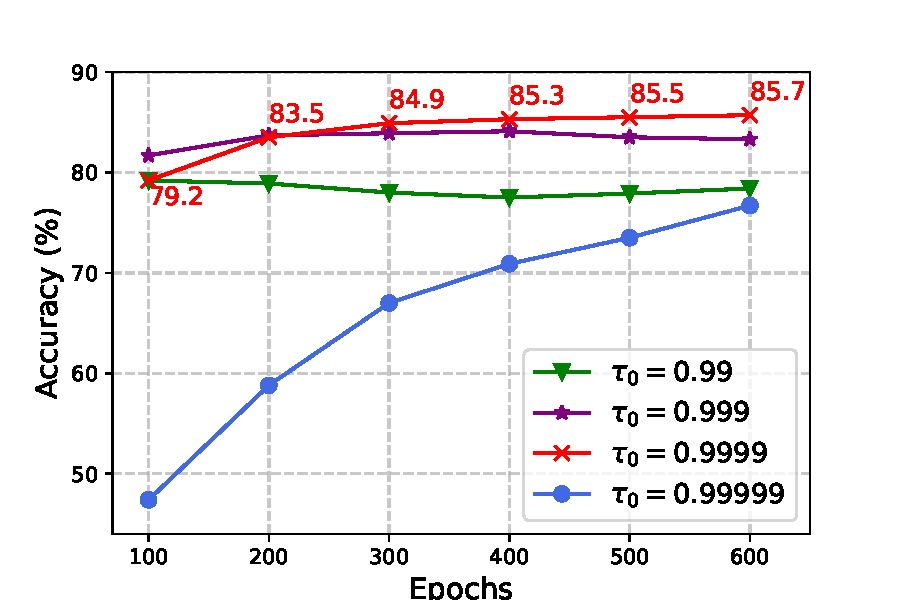
\includegraphics[width=0.95\linewidth]{figures/ema_ablation.pdf}
%   \caption{
%     Ablation study on the EMA parameter $\tau_{0}$.
%     The results are reported on the NTU-60 XSub dataset under the
%     linear protocol.
%   }
%   \label{fig:ema_ablation}
% \end{figure}

% \begin{figure}[tb]
%   \centering
%   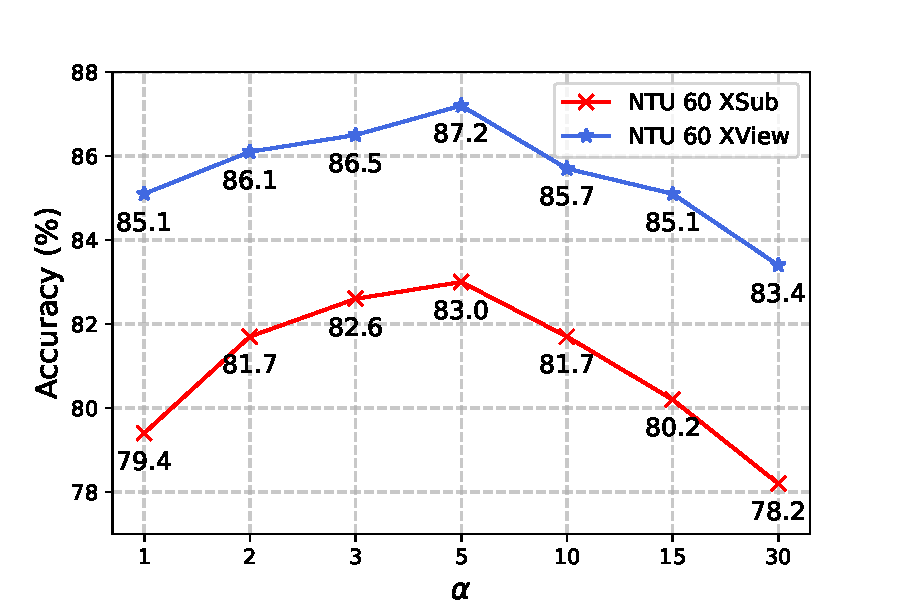
\includegraphics[width=0.95\linewidth]{figures/alpha_ablation.pdf}
%   \caption{
%     Ablation study on the tube length.
%     $\alpha=0$ is equivalent to random masking, while $\alpha=30$, which is the length
%     of the input sequence, is equivalent to single-tube masking.
%   }
%   \label{fig:alpha_ablation}
% \end{figure}

\begin{figure}[htbp]
  \begin{minipage}[b]{0.49\linewidth}
    \centering
    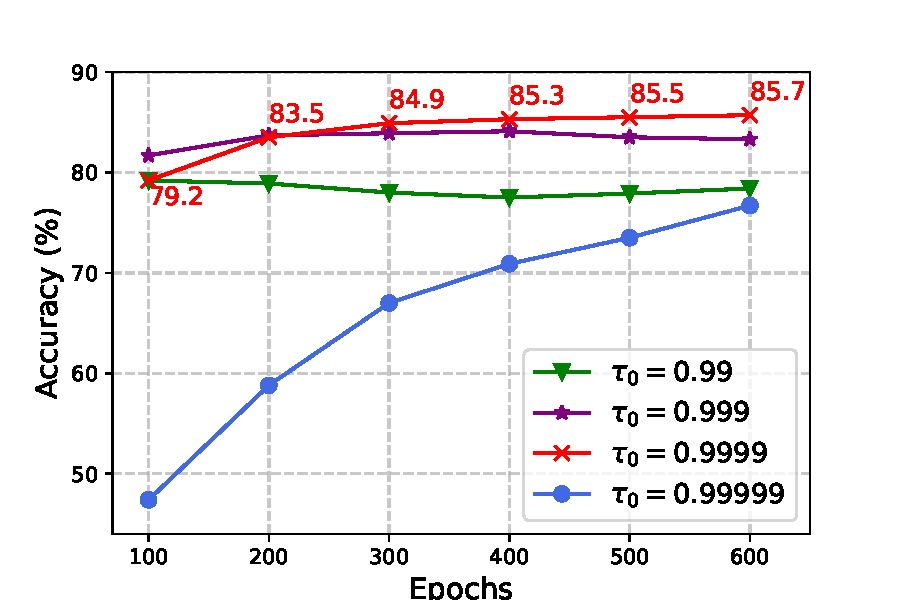
\includegraphics[width=0.95\linewidth]{figures/ema_ablation.pdf}
    \caption{Ablation study on the EMA parameter $\tau_{0}$. The results are reported on the NTU-60 XSub dataset under the linear protocol.}
    \label{fig:ema_ablation}
  \end{minipage}
  \hfill
  \begin{minipage}[b]{0.49\linewidth}
    \centering
    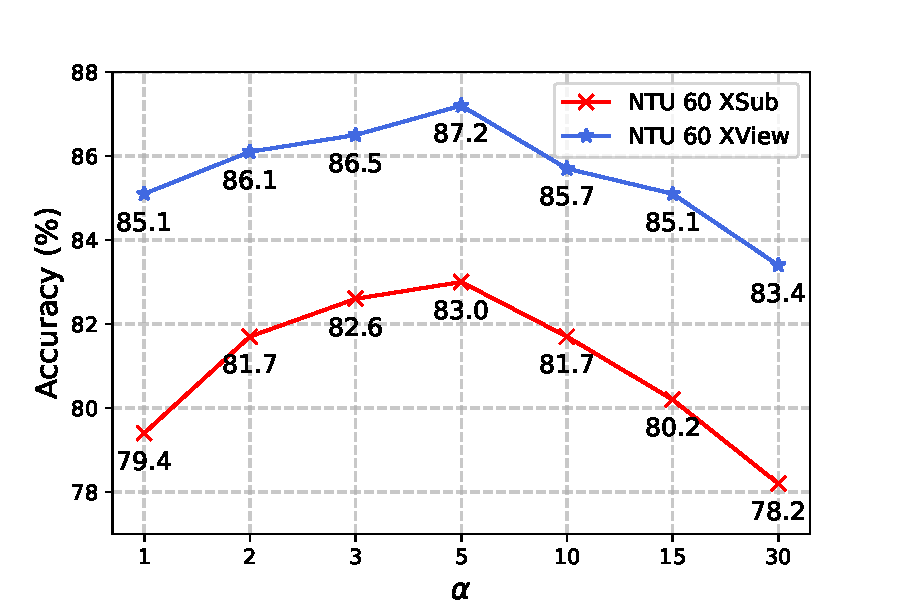
\includegraphics[width=0.95\linewidth]{figures/alpha_ablation.pdf}
    \caption{Ablation study on the tube length. $\alpha=0$ is equivalent to random masking, while $\alpha=30$, which is the length of the input sequence, is equivalent to single-tube masking.}
    \label{fig:alpha_ablation}
  \end{minipage}
\end{figure}

% \begin{figure}[tb]
%   \centering
%   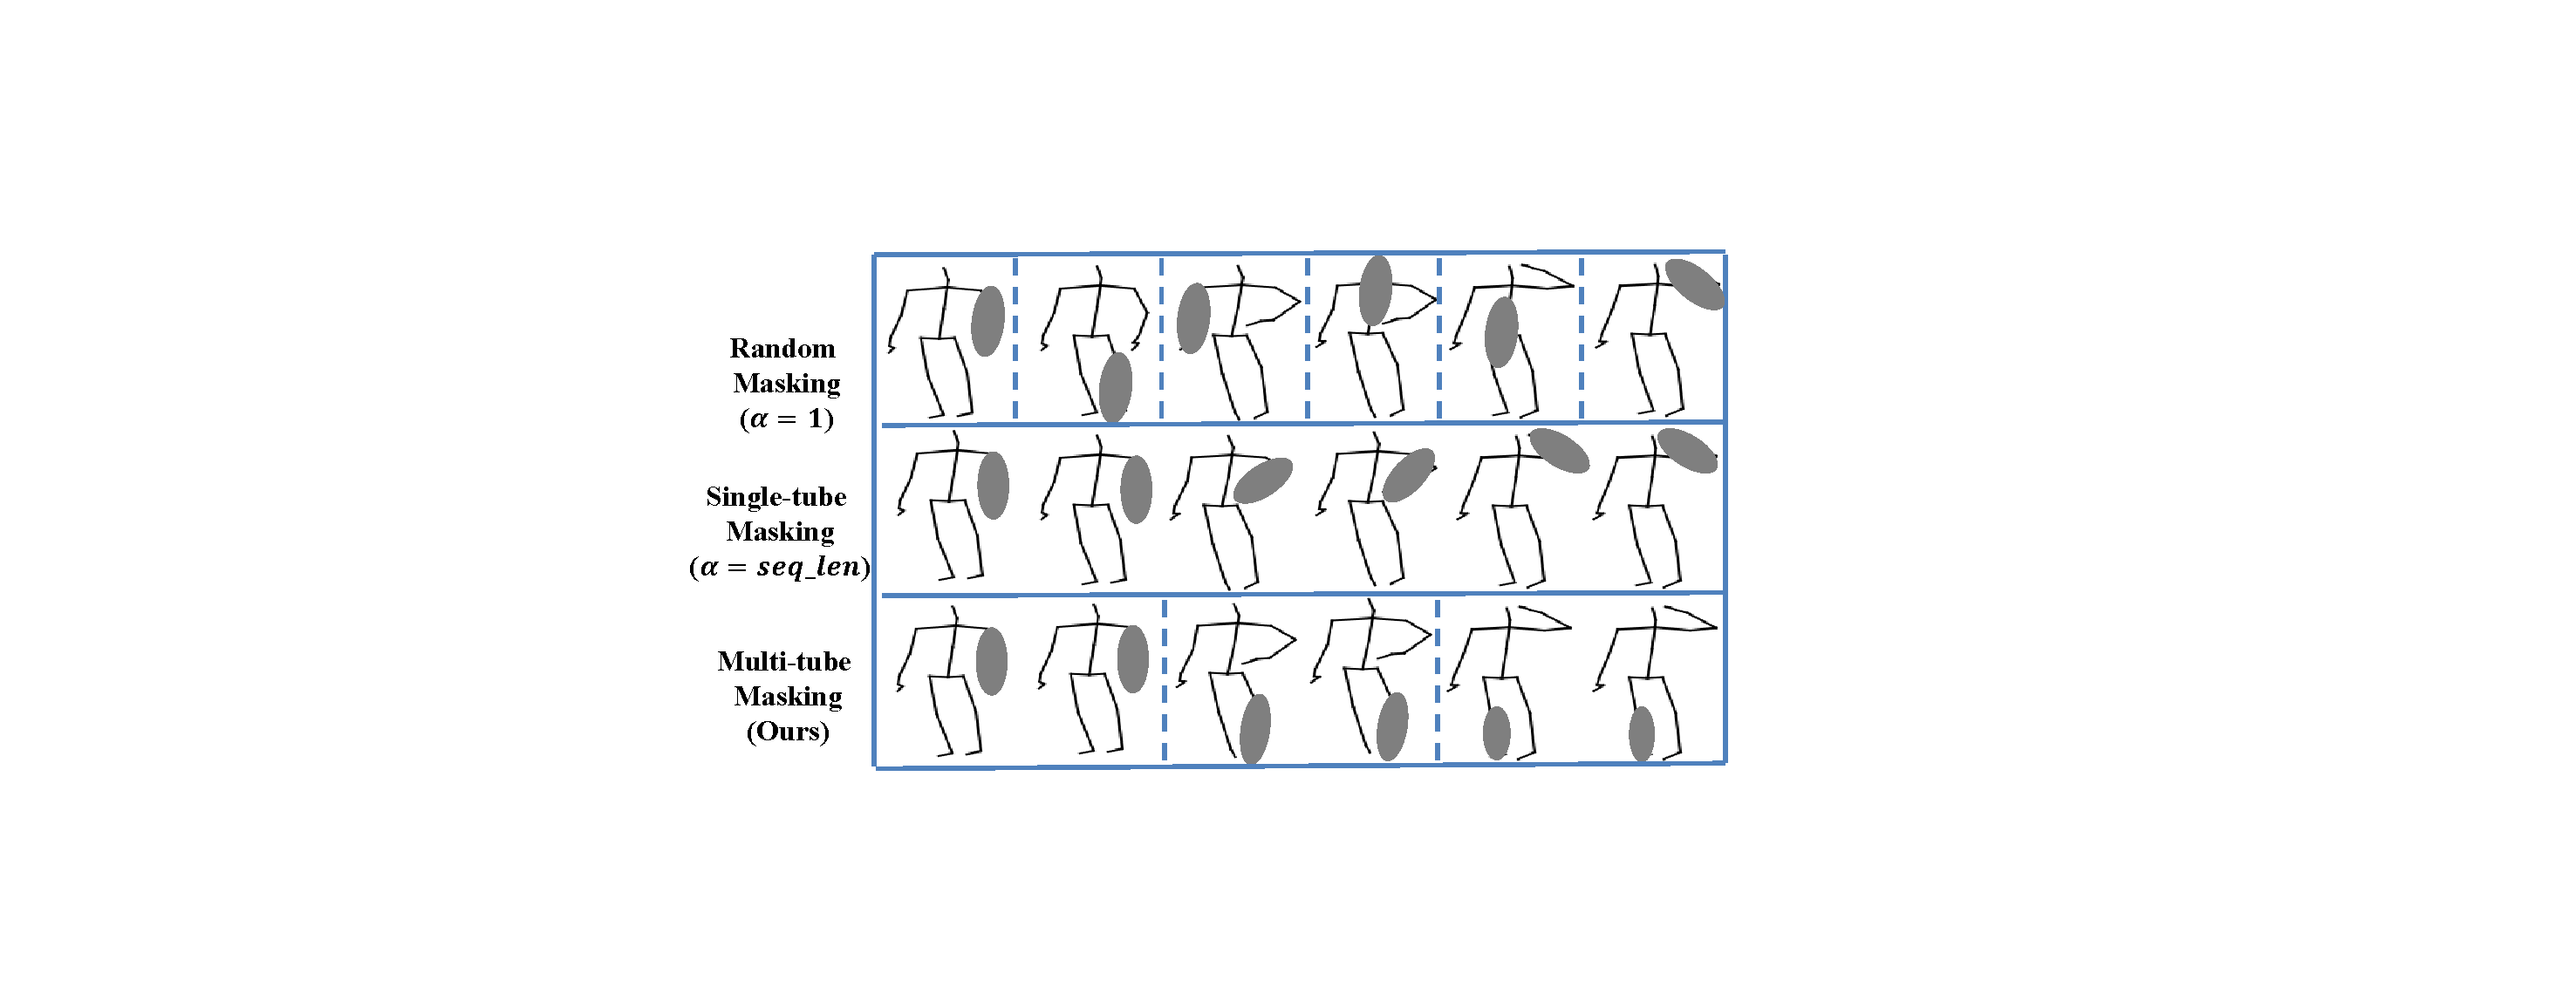
\includegraphics[width=0.95\linewidth]{figures/fig_masking.pdf}
%   \caption{
%     Demonstration of various masking strategies.
%     The grey areas represent the masked parts of the body
%   }
%   \label{fig:masking_demo}
% \end{figure}

% \begin{table}[tb]
%     \centering
%     \begin{tabular}{c@{\hspace{6pt}}c c c c}
%       \toprule
%       \multirow{2}{*}{Strategy} &
%       \multirow{2}{*}{$\alpha$} &
%       \multirow{2}{*}{$\beta$} &
%       \multicolumn{2}{c}{NTU 60} \\
%       & & & XSub & XView \\
%       \midrule
%       Random & 1 & 0.0 & 79.4 & 85.1 \\
%       Single-tube & 30 & 0.0 & 78.2 & 83.4 \\
%       Multi-tube & 5 & 0.0 & 83.0 & 87.2 \\
%       \textbf{MAMT(Ours)} & 5 & 0.1 & \textbf{83.5} & \textbf{87.7} \\
%       \bottomrule
%     \end{tabular}
%     \caption{
%       Ablation study on the masking strategy.
%       $\alpha$ represents the length of each tube, while $\beta$ denotes the
%       parameter of motion-aware sampling.
%     }
%     \label{tab:masking_strategy}
% \end{table}

% \begin{figure}[tb]
%   \begin{minipage}[b]{0.51\linewidth}
%     \centering
%     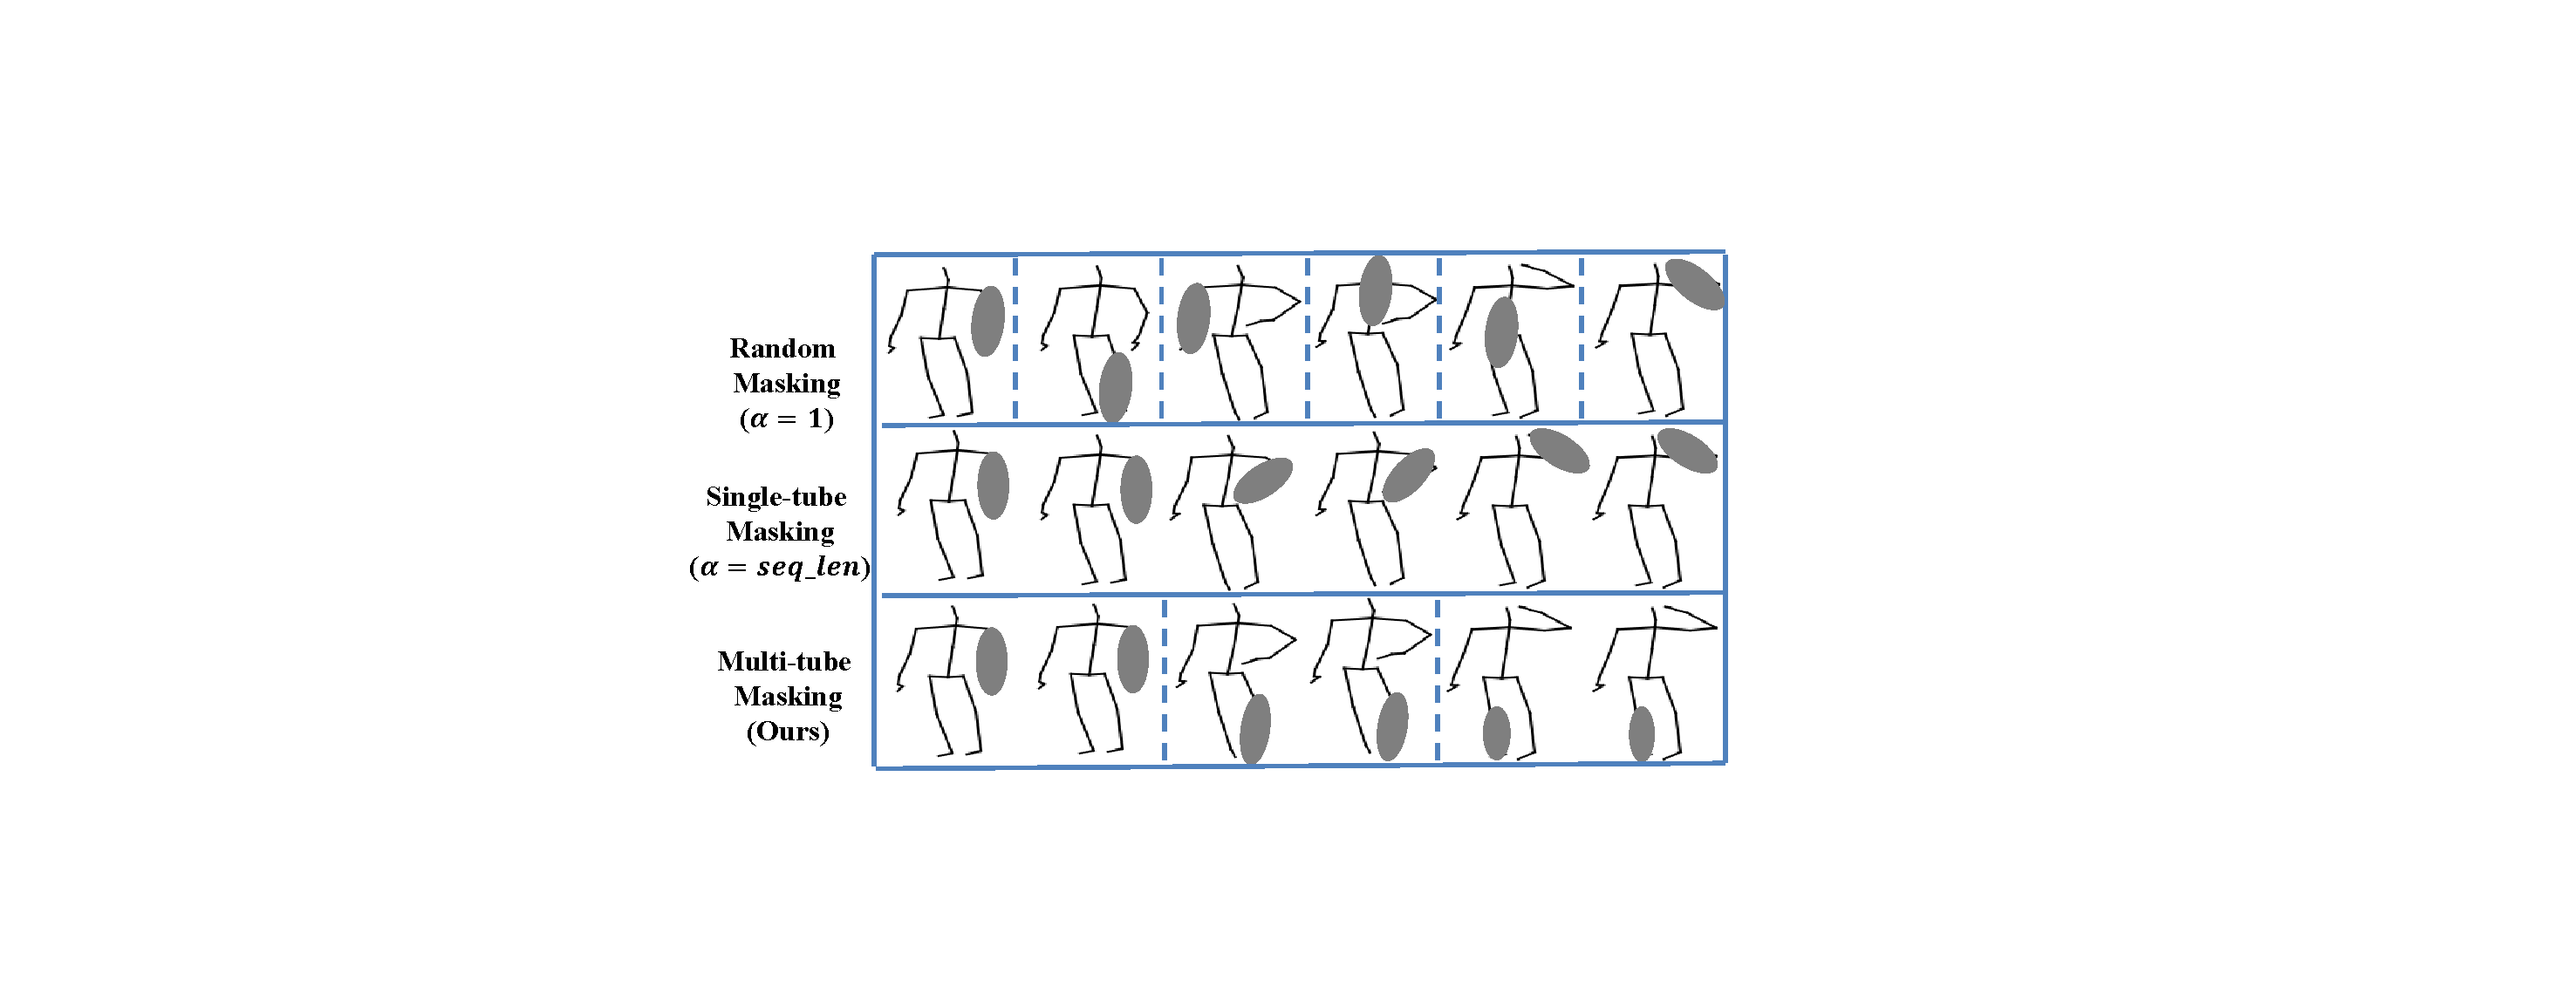
\includegraphics[width=\linewidth]{figures/fig_masking.pdf}
%     \caption{Demonstration of various masking strategies. The grey areas represent the masked parts of the body}
%     \label{fig:masking_demo}
%   \end{minipage}%
%   \hfill
%   \begin{minipage}[b]{0.48\linewidth}
%     \centering
%     \begin{tabular}{c c c c c}
%       \toprule
%       \multirow{2}{*}{Strategy} &
%       \multirow{2}{*}{$\alpha$} &
%       \multirow{2}{*}{$\beta$} &
%       \multicolumn{2}{c}{NTU 60} \\
%       & & & XSub & XView \\
%       \midrule
%       Random & 1 & 0.0 & 79.4 & 85.1 \\
%       Single-tube & 30 & 0.0 & 78.2 & 83.4 \\
%       Multi-tube & 5 & 0.0 & 83.0 & 87.2 \\
%       \textbf{MAMT(Ours)} & 5 & 0.1 & \textbf{83.5} & \textbf{87.7} \\
%       \bottomrule
%     \end{tabular}
%     \captionof{table}{Ablation study on the masking strategy. $\alpha$ represents the length of each tube, while $\beta$ denotes the parameter of motion-aware sampling.}
%     \label{tab:masking_strategy}
%   \end{minipage}
% \end{figure}

% \begin{table}[tb]
%     \centering
%     \begin{subtable}[t]{0.495\linewidth}
%       \begin{tabular}{c c c}
%         \toprule
%         \multirow{2}{*}{$\beta$} &
%         \multicolumn{2}{c}{NTU 60} \\
%         & XSub & XView \\
%         \midrule
%         0.0 & 83.0 & 87.2 \\
%         0.1 & \textbf{83.5} & \textbf{87.7} \\
%         0.2 & 82.1 & 87.0 \\
%         0.3 & 79.5 & 86.3 \\
%         \bottomrule
%       \end{tabular}
%       \caption{
%         Motion-aware sampling
%       }
%       \label{tab:beta}
%     \end{subtable}
%     \begin{subtable}[t]{0.495\linewidth}
%       \begin{tabular}{c c c}
%         \toprule
%         \multirow{2}{*}{$m$} &
%         \multicolumn{2}{c}{NTU 60} \\
%         & XSub & XView \\
%         \midrule
%         0.80 & 83.1 & 86.7 \\
%         0.85 & 83.3 & 87.3 \\
%         0.90 & \textbf{83.5} & \textbf{87.7} \\
%         0.95 & 77.1 & 82.1 \\
%         \bottomrule
%       \end{tabular}
%       \caption{
%         Masking ratio
%       }
%       \label{tab:masking_ratio}
%   \end{subtable}
%   \caption{
%     Ablation study on the masking ratio and motion-aware sampling.
%   }
%   \label{tab:masking_ratio_and_beta}
% \end{table}

% \begin{figure}[tb]
%     \begin{minipage}[t]{0.5\linewidth}
%         \centering
%         \begin{tabular}{c c c c c}
%           \toprule
%           \multirow{2}{*}{Strategy} &
%           \multirow{2}{*}{$\alpha$} &
%           \multirow{2}{*}{$\beta$} &
%           \multicolumn{2}{c}{NTU 60} \\
%           & & & XSub & XView \\
%           \midrule
%             Random & 1 & 0.0 & 79.4 & 85.1 \\
%             Single-tube & 30 & 0.0 & 78.2 & 83.4 \\
%             Multi-tube & 5 & 0.0 & 83.0 & 87.2 \\
%             \textbf{MAMT(Ours)} & 5 & 0.1 & \textbf{83.5} & \textbf{87.7} \\
%           \bottomrule
%         \end{tabular}
%         % \captionsetup{width=0.8\linewidth}
%         \captionof{table}{Masking strategy.}
%         \label{tab:masking_strategy}
%     \end{minipage}
%     \hfill
%     \begin{minipage}[t]{0.24\linewidth}
%         \centering
%         \begin{tabular}{c c c}
%             \toprule
%             \multirow{2}{*}{$\beta$} &
%             \multicolumn{2}{c}{NTU 60} \\
%             & XSub & XView \\
%             \midrule
%             0.0 & 83.0 & 87.2 \\
%             0.1 & \textbf{83.5} & \textbf{87.7} \\
%             0.2 & 82.1 & 87.0 \\
%             0.3 & 79.5 & 86.3 \\
%             \bottomrule
%         \end{tabular}
%         % \captionsetup{width=0.8\linewidth}
%         \captionof{table}{Motion-aware sampling}
%         \label{tab:beta}
%     \end{minipage}
%     \hfill
%     \begin{minipage}[t]{0.24\linewidth}
%         \centering
%         \begin{tabular}{c c c}
%             \toprule
%             \multirow{2}{*}{$m$} &
%             \multicolumn{2}{c}{NTU 60} \\
%             & XSub & XView \\
%             \midrule
%             0.80 & 83.1 & 86.7 \\
%             0.85 & 83.3 & 87.3 \\
%             0.90 & \textbf{83.5} & \textbf{87.7} \\
%             0.95 & 77.1 & 82.1 \\
%             \bottomrule
%         \end{tabular}
%         % \captionsetup{width=0.8\linewidth}
%         \captionof{table}{Masking ratio}
%         \label{tab:masking_ratio}
%     \end{minipage}
%     \caption{
%       Ablation study on the Motion-Aware Multi-Tube (MAMT) masking strategy.
%       $\alpha$ represents the length of each tube, while $\beta$ denotes the parameter of motion-aware sampling.
%       $m$ denotes the masking ratio.
%     }
%     \label{tab:masking_ratio_and_beta}
% \end{figure}

\begin{figure}[tb]
    \captionof{table}{Ablation study on the \textbf{Motion-Aware Multi-Tube (MAMT)} masking strategy. $\alpha$ represents the length of each tube, while $\beta$ denotes the parameter of motion-aware sampling. $m$ denotes the masking ratio.}
    \centering
    \begin{subfigure}[t]{0.5\linewidth}
        \centering
        \begin{tabular}{c c c c c}
            \toprule
            \multirow{2}{*}{Strategy} & \multirow{2}{*}{$\alpha$} & \multirow{2}{*}{$\beta$} & \multicolumn{2}{c}{NTU 60} \\
            & & & XSub & XView \\
            \midrule
            Random & 1 & 0.0 & 79.4 & 85.1 \\
            Single-tube & 30 & 0.0 & 78.2 & 83.4 \\
            Multi-tube & 5 & 0.0 & 83.0 & 87.2 \\
            \textbf{MAMT(Ours)} & 5 & 0.1 & \textbf{83.5} & \textbf{87.7} \\
            \bottomrule
        \end{tabular}
        \caption{Masking strategy.}
        \label{tab:masking_strategy}
    \end{subfigure}
    \hfill
    \begin{subfigure}[t]{0.24\linewidth}
        \centering
        \begin{tabular}{c c c}
            \toprule
            \multirow{2}{*}{$\beta$} & \multicolumn{2}{c}{NTU 60} \\
            & XSub & XView \\
            \midrule
            0.0 & 83.0 & 87.2 \\
            0.1 & \textbf{83.5} & \textbf{87.7} \\
            0.2 & 82.1 & 87.0 \\
            0.3 & 79.5 & 86.3 \\
            \bottomrule
        \end{tabular}
        \caption{Motion-aware sampling}
        \label{tab:beta}
    \end{subfigure}
    \hfill
    \begin{subfigure}[t]{0.24\linewidth}
        \centering
        \begin{tabular}{c c c}
            \toprule
            \multirow{2}{*}{$m$} & \multicolumn{2}{c}{NTU 60} \\
            & XSub & XView \\
            \midrule
            0.80 & 83.1 & 86.7 \\
            0.85 & 83.3 & 87.3 \\
            0.90 & \textbf{83.5} & \textbf{87.7} \\
            0.95 & 77.1 & 82.1 \\
            \bottomrule
        \end{tabular}
        \caption{Masking ratio}
        \label{tab:masking_ratio}
    \end{subfigure}
    \label{tab:masking_ratio_and_beta}
\end{figure}

\noindent \textbf{Masking Strategy:}
\cref{tab:masking_strategy} illustrates the effectiveness of our proposed
motion-aware tube masking strategy. We compared its performance with random masking
and tube masking (without motion-aware sampling). The results indicate a significant
performance boost with tube masking compared to random masking, showing improvements
of 3.6\% and 2.1\% under the XSub and XView testing protocols of the NTU-60 dataset,
respectively. This underscores the capability of tube segmentation to compel the
model into effective long-range motion modeling. Moreover, motion-aware tube masking
further improves performance, highlighting the value of guiding the model to focus
on semantically rich action regions. A detailed analysis of hyperparameters in
motion-aware tube masking will be presented in subsequent sections.

\noindent \textbf{Tube Length:}
We investigated the impact of the length $\alpha$ of each tube on pre-training performance.
As depicted in \cref{fig:alpha_ablation}, excessively short tube lengths result
in information leakage between adjacent frames, leading to a performance decline.
On the other hand, overly long tube lengths pose excessively challenging pre-training
tasks, impairing the model's learning capacity, as discussed in \cref{sec:motion-aware_tube_masking}.
Hence, selecting an appropriate tube length is crucial. Considering the results
from \cref{fig:alpha_ablation}, we identified a tube length of $\alpha=5$ as
optimal, achieving the best balance and performance.

\noindent \textbf{Motion-aware Sampling:}:
We compared the performance of learned representations under different motion-aware
sampling parameters $\beta$. As shown in \cref{tab:beta}, selecting an appropriate
sampling parameter enhances pre-training performance compared to not using
motion prior information ($\beta=0$). However, excessively large sampling parameters
can result in overly fixed sampling of joints, leading to a loss of diversity and
a subsequent performance decline. We empirically found that a sampling parameter of
$\beta=0.1$ yields the best results.

\noindent \textbf{Masking Ratio:}:
In \cref{tab:masking_ratio}, we compared the influence of different masking ratios
on the results. It is evident that excessively large or small masking ratios can
impair the final performance. We ultimately selected a masking ratio of 90\% to
achieve optimal results.